\section{Algoritmos para la detección de rostros y extracción de características}

Dentro del pipeline de reconocimiento facial, la detección y la extracción de embeddings son etapas críticas que se benefician de algoritmos especializados.\\

En este trabajo se prestara especial interés en el algoritmo MTCNN para la detección de rostros y FaceNet para la obtención de embeddings.


\subsection{MTCNN (Multitask Cascaded Convolutional Networks)}


\begin{figure}[htbp]
	\begin{center}
		\fbox{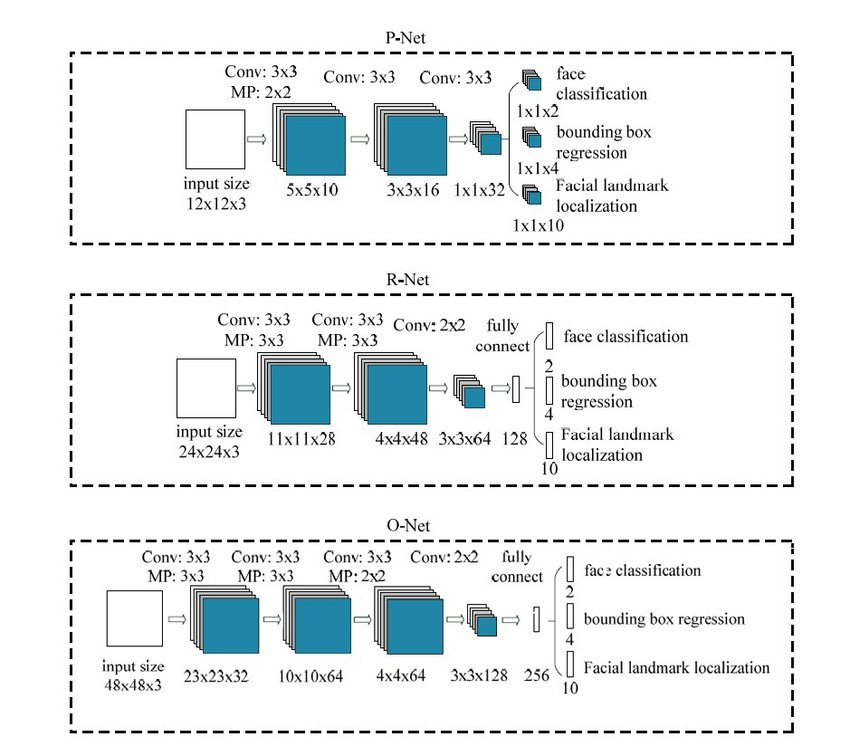
\includegraphics[width=.68\textwidth]{images/mtcnn_architecture}}
		\caption{Arquitectura de MTCNN. \cite{MTCNN_Paper}.}
		\label{fig:Arquitectura de MTCNN}
	\end{center}
\end{figure}


\subsubsection{Antecedentes}

Cuando MTCNN (Multitask Cascaded Convolutional Networks) apareció en escena en 2016, con una presentación más formal en la conferencia ICCV de 2017, rápidamente se convirtió en un referente para la detección facial. ¿Por qué? Porque logra algo que, en ese momento, era un gran avance: combinar la detección de rostros y la alineación de puntos clave faciales en un solo proceso eficiente. En lugar de depender de modelos separados para cada tarea, MTCNN las integra en un pipeline único, lo que reduce significativamente el costo computacional \cite{MTCNN_Paper}.\\


\subsubsection{Arquitectura en Cascada: PNet, RNet, ONet}

MTCNN emplea una estructura en cascada compuesta por tres redes neuronales convolucionales (CNNs) que colaboran para refinar progresivamente las propuestas de rostros y detectar los puntos clave \cite{MTCNN_Paper}.\\

Dada esta naturaleza en forma de cascada es que se da lugar a un refinamiento progresivo, iniciando con una detección general y avanzando hacia una alineación más precisa.\\

A continuación, se presenta una breve descripción sobre las redes neuronales que conforman a MTCNN \cite{MTCNN_Paper}:

\begin{enumerate}
	
	
	\item \textbf{PNet (Proposal Network)}:  Esta es la red inicial que escanea la imagen en diferentes escalas para generar regiones candidatas de rostros, representadas por cuadros delimitadores. Su función es identificar posibles ubicaciones de rostros de manera eficiente.\\
	
	\item \textbf{RNet (Refinement Network)}: RNet toma las regiones candidatas de rostros generadas por PNet, las refina filtrando los falsos positivos y ajusta aún más los cuadros delimitadores. Esta etapa mejora la precisión de las detecciones iniciales.\\
	
	\item \textbf{ONet (Output Network)}: Como etapa final, ONet refina aún más los cuadros delimitadores y detecta cinco puntos clave faciales: los ojos, la nariz y las comisuras de la boca. Esta red proporciona la salida final de la detección y alineación. 
	
\end{enumerate}


\subsection{FaceNet}

\subsubsection{Visión general}

FaceNet es un sistema de reconocimiento facial desarrollado por investigadores de Google, presentado por primera vez en la Conferencia IEEE sobre Visión por Computadora y Reconocimiento de Patrones de 2015. Su concepto central es aprender un mapeo, o embedding, directamente desde un conjunto de imágenes faciales a un espacio euclidiano de 128 dimensiones \cite{FaceNet_Paper}.\\

Una vez que se encuentran los emebddings en este espacio vectorial, su similitud se determina calculando la distancia euclidiana entre los embeddings que se estén comparando.\\

Además de proporcionar un marco de trabajo para la generación de embeddings de calidad, FaceNet también puede ser usado para crear clusters de personas, lo que lo convierte en un modelo sencillo de entender y robusto hasta la fecha \cite{FaceNet_Paper}.


\begin{figure}[htbp]
	\begin{center}
		\fbox{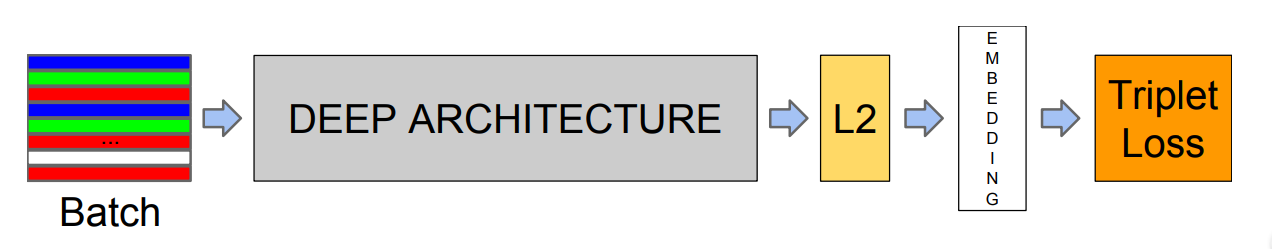
\includegraphics[width=.68\textwidth]{images/facenet_architecture}}
		\caption{Arquitectura general de FaceNet. \cite{FaceNet_Paper}.}
		\label{fig:Arquitectura general de FaceNet}
	\end{center}
\end{figure}




\subsubsection{Función de pérdida por tripletas (Triplet Loss)}

La principal aportación de este modelo con respecto a otros es la implementación de un proceso de aprendizaje basado en Tripletas. 
Una tripleta hace referencia a un conjunto de tres imágenes, una imagen base, una positiva y una negativa en donde la imagen base es una imagen del rostro de una persona cualquiera, la imagen positiva es una imagen distinta de la misma persona base y, la imagen negativa, es una imagen de una persona distinta a la persona base \cite{FaceNet_Paper}.\\

Esta función está diseñada para asegurar que los embeddings de la misma persona estén muy cerca entre sí en el espacio vectorial, mientras que los embeddings de personas diferentes estén lo suficientemente lejos \cite{FaceNet_Paper}.\\

Esta optimización directa del espacio de embedding para el cálculo de similitud es lo que permitió la alta precisión de FaceNet y su influencia en modelos posteriores basados en embeddings \cite{L16}.\\ 




\begin{figure}[htbp]
	\begin{center}
		\fbox{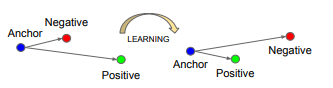
\includegraphics[width=.50\textwidth]{images/triplet_loss}}
		\caption{Aprendizaje basado en tripletas. \cite{FaceNet_Paper}.}
		\label{fig:Aprendizaje basado en tripletas}
	\end{center}
\end{figure}


\subsubsection{CASIA-WebFace}

El conjunto de datos CASIA WebFace fue introducido en el trabajo "Learning Face Representation from Scratch" y surgió como una necesidad de contar con conjuntos de datos a gran escala para el entrenamiento de modelos de aprendizaje profundo ya que, este tipo de sistemas requieren de una gran cantidad de datos etiquetados \cite{CASIA}.\\

La principal ventaja de contar con conjuntos de datos grandes como este es la oportunidad que brindan para que nuevas arquitecturas aprendan a identificar y representar los rostros directamente desde cero, eliminando la dependencia de características manuales o los sesgos que pueden acarrear los modelos pre-entrenados \cite{CASIA}.\\


Algunas de las características importantes de este conjunto de datos son \cite{CASIA}.:

\begin{itemize}
	
	\item \textbf{Tamaño}:\\ 
	
	Es un conjunto de datos de gran tamaño en comparación con otros como LFW ya que su principal propósito es ser utilizado para el entrenamiento de modelos robustos. Por lo tanto, contiene aproximadamente 500 mil imágenes de rostros de un total de 10,575 personas extraídas directamente de la web.\\
	
	\item \textbf{Adquisición de imágenes}\\	
	
	Como su propio nombre lo sugiere, las imágenes que conforman a este conjunto de datos fueron obtenidas a través de la web, por lo que presentan una gran variabilidad en las condiciones en las que fueron tomadas, por ejemplo:
	
	\begin{itemize}
		
		\item \textbf{Iluminación}: Diferentes condiciones de luz (día, noche, sombras, reflejos).\\
		
		\item \textbf{Pose}: Varias poses de la cabeza (frontal, perfil, semi-perfil, inclinaciones).\\
		
		\item \textbf{Expresión} Diversas expresiones faciales (neutra, feliz, triste, enojada, etc.).\\		
		
		\item \textbf{Oclusión} Posibles oclusiones parciales del rostro (gafas, cabello, objetos).\\	
		
		\item \textbf{Fondo Fondos no controlados y variables, lo que añade complejidad.}\\
		
		\item \textbf{Calidad de imagen} Las imágenes varían en resolución, nitidez y compresión.
		\\				
			
		
	\end{itemize}
	
	
	\item \textbf{Uso}: Dado el tamaño de este conjunto de datos, es posible usarlo para una variedad de tareas dentro del flujo de trabajo de un sistema de reconocimiento facial, por ejemplo, puede usarse para entrenar modelos basados en arquitecturas de redes neuronales profundas y, por otro lado, es posible usar una parte de este para evaluar el rendimiento de modelos que hayan sido entrenados con conjuntos de datos diferentes.\\
	
	
\end{itemize}

\begin{figure}[htbp]
	\begin{center}
		\fbox{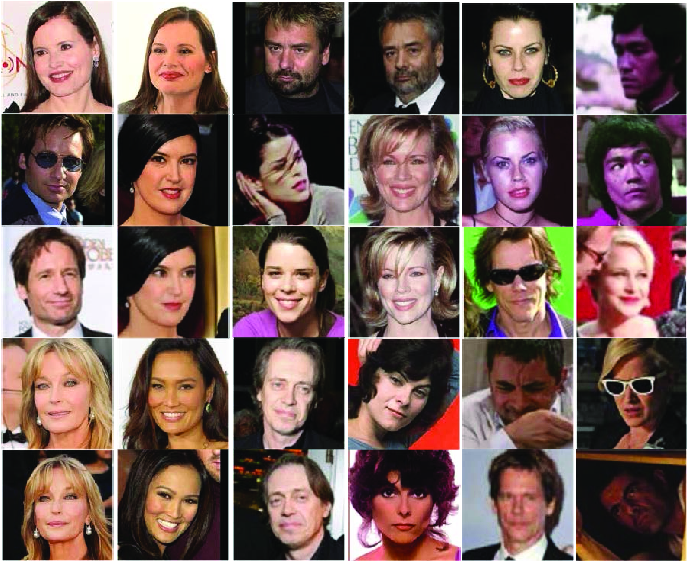
\includegraphics[width=.50\textwidth]{images/casia_subset}}
		\caption{Conjunto de datos CASIA WebFace. \cite{CASIA}.}
		\label{fig:Conjunto de datos CASIA WebFace}
	\end{center}
\end{figure}


\subsubsection{Labeled Face in the Wild}

Este conjunto de datos fue creado y mantenido por investigadores de la Universidad de Massachusetts, Amherst y se introdujo en el año 2007.
Actualmente, su importancia radica en su papel como punto de referencia para evaluar  el rendimiento de algoritmos de reconocimiento facial en condiciones no controladas o como sus propios autores mencionan, en la naturaleza \cite{LFW}.\\

Sin embargo, a pesar de estar intrínsecamente relacionado con el reconocimiento facial, este conjunto de datos suele usarse especialmente al trabajar el problema de la verificación facial que como se explico anteriormente, consiste en decidir si dos imágenes pertenecen a la misma persona \cite{LFW}.\\

Dentro de los puntos que diferencian a este conjunto de datos con respecto a otros se destacan los siguientes \cite{LFW}:


\begin{itemize}
	
	\item \textbf{Tamaño} Contiene aproximadamente 13,233 imágenes de rostros de 5,749 personas únicas. A diferencia de CASIA WebFace, LFW es significativamente más pequeño en términos de número de imágenes y, sobre todo, en el número de identidades.\\
	
	\item \textbf{Adquisición de imágenes} El origen de las imágenes que conforman al conjunto de datos es la web, por lo que trae consigo una gran variabilidad y desafíos para el reconocimiento facial como variación intra-clase alta, casos de variación de pose, iluminación y oclusión y la presencia de fondos complejos.\\
	
	\item \textbf{Estructura para evaluación}  LFW es conocido por su protocolo de evaluación estándar para la verificación facial. Este protocolo define 6,000 pares de imágenes, de los cuales 3000 pares son de la misma persona, 3000 pares son de personas distintas.\\
	
	\item \textbf{Uso} Se utiliza principalmente como un marco de referencia para la evaluación de tareas de verificación facial y, comparación de algoritmos de reconocimiento facial.\\
	
\end{itemize}


\begin{figure}[htbp]
	\begin{center}
		\fbox{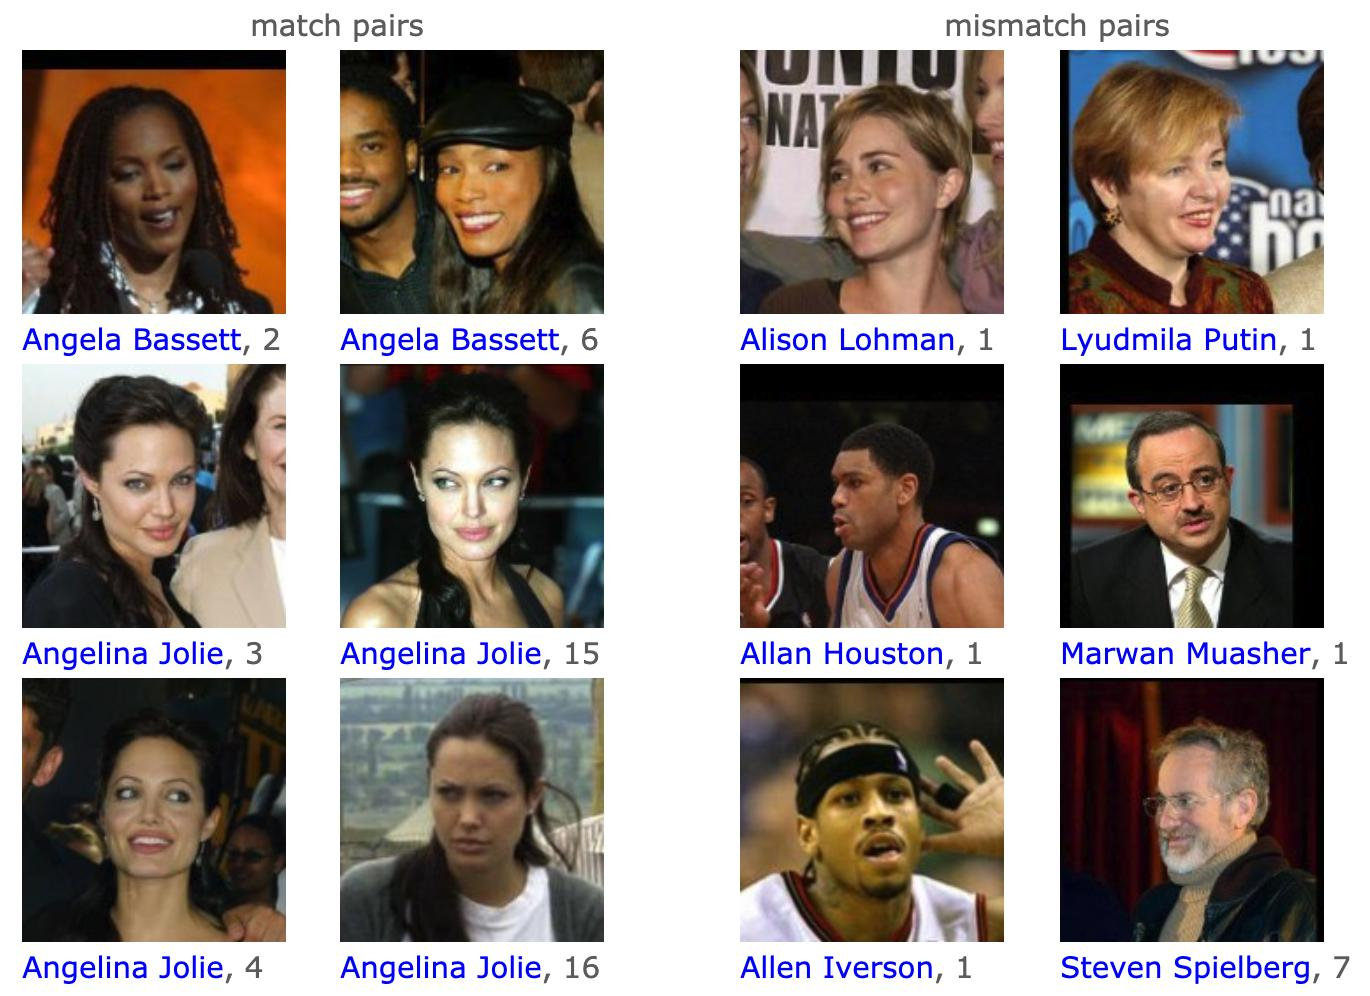
\includegraphics[width=.50\textwidth]{images/lfw_subset}}
		\caption{Algunos pares en el conjunto LFW. \cite{LFW}.}
		\label{fig:Algunos pares en el conjunto LFW}
	\end{center}
\end{figure}


\begin{figure}[htbp]
	\begin{center}
		\fbox{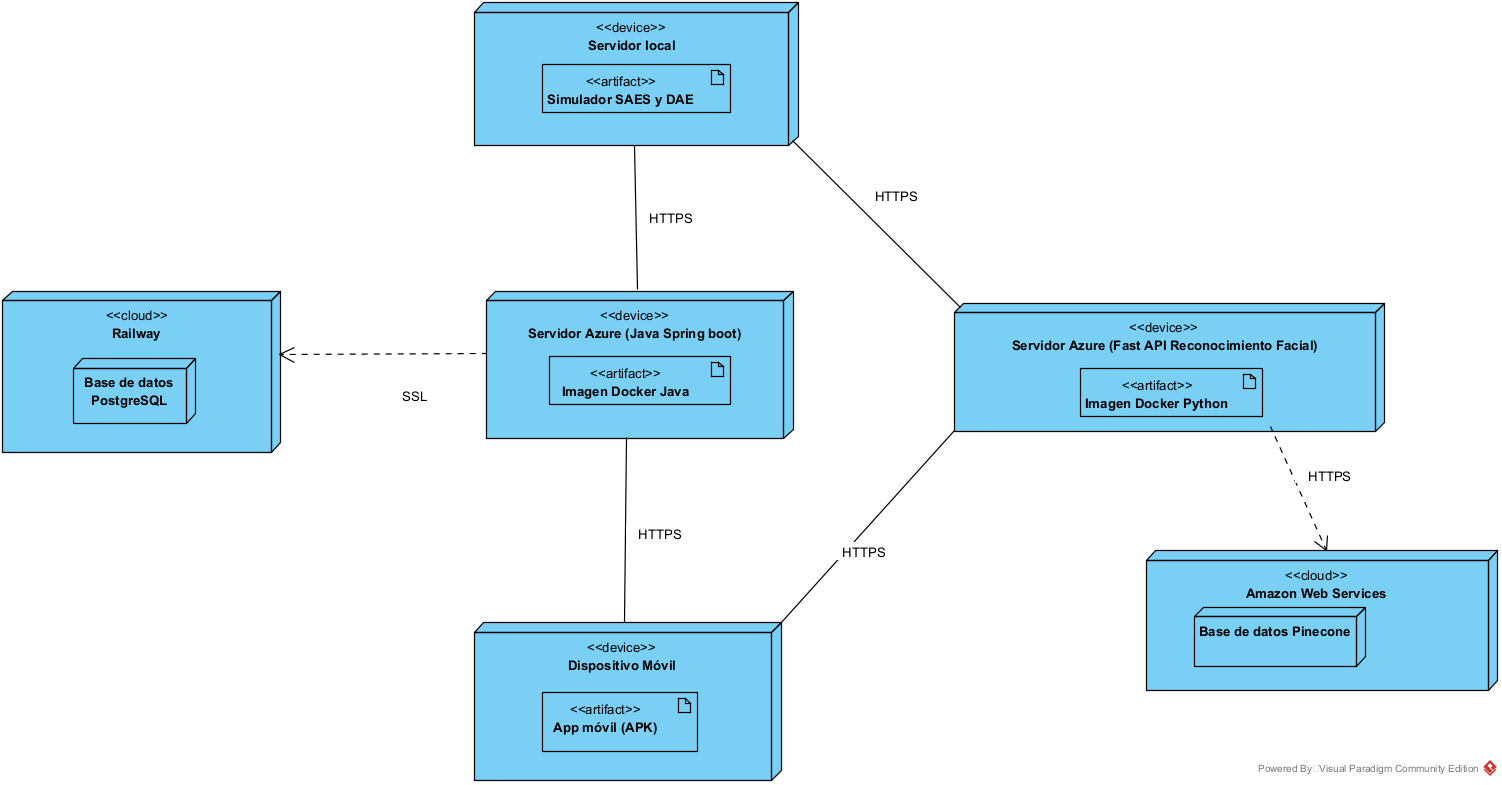
\includegraphics[width=.70\textwidth]{images/diagrama_despliegue}}
		\caption{Algunos pares en el conjunto LFW. \cite{LFW}.}
		\label{fig:Algunos pares en el conjunto LFW}
	\end{center}
\end{figure}